
% \begin{longtable}{|>{\raggedright\arraybackslash}m{0.17\textwidth}|>{\raggedright\arraybackslash}m{0.2\textwidth}|>{\raggedright\arraybackslash}m{0.2\textwidth}|>{\raggedright\arraybackslash}m{0.35\textwidth}|}
%     \hline
%     \textbf{Function} & \textbf{Test Case} & \textbf{Test Data} & \textbf{Expected Output} \\ \hline
%     parse\_font\_file & empty filename & filename="" & Error message: "Filename is empty" \\ \hline
%     parse\_font\_file & fopen() fails & filename="font.exe" & Error message: "unable to open file" \\ \hline
%     parse\_font\_file & memory allocation fails & Simulate malloc failure  &  Error message: "Memory allocation failed" \\ \hline
%     parse\_font\_file & normal case & filename= "SingleStrokeFont.txt" &  normal operation: calls hash\_table\_insert(), 128 times \\ \hline
%     hash\_table\_insert & NULL hastable & hash\_table=NULL & Error message: "Hash table is NULL" \\ \hline
%     hash\_table\_insert & NULL character & character=NULL & Error message: "Character is NULL" \\ \hline
%     hash\_table\_insert & memory allocation fails & Simulate malloc failure  &  Error message: "Memory allocation failed" \\ \hline
%     hash\_table\_insert & normal case & ascii\_key=0, character=fontCharacter\_t &  normal operation: inserts fontCharacter into hash table \\ \hline
%     hash\_table\_insert & insert multiple characters & insert 'A', 'B', 'C' &  normal operation: inserts fontCharacter into hash table \\ \hline
%     hash\_table\_insert & confirm correct operation with hash\_table\_lookup & *font\_char = hash\_table\_lookup( font\_data, key) & font\_char$->$ascii\_key == Key \\ \hline
%     hash\_table\_lookup & NULL hastable & hash\_table=NULL & Error message: "Hash table is NULL" \\ \hline
%     hash\_table\_lookup & normal case & ascii\_key=0 &  normal operation: returns fontCharacter from hash table with key 0\\ \hline
%     hash\_table\_lookup & look up character that doesnt exist & ascii\_key=999 &  Error message: "Character not found" \\ \hline
%     scale\_font\_data & NULL font\_data & font\_data=NULL & Error message: "Font data is NULL" \\ \hline
%     scale\_font\_data & input not between 4-10mm & 11 & Error message: "Input not between 4-10mm" \\ \hline
%     scale\_font\_data & test with 'A' 4mm & \footnotesize$\begin{array}{ccc}
%         999 &65 &6 \\
%         0 &0 &0\\
%         6 &18& 1\\
%         12 &0& 1\\
%         3 &9& 0\\
%         9& 9& 1\\
%         18 &0& 0\\
%         \end{array}$ & \footnotesize$\begin{array}{ccc}
%         999 &65 &6 \\
%         0 &0 &0\\
%         1.33 &4.00& 1\\
%         2.67 &0& 1\\
%         0.67 &2.00& 0\\
%         2.00& 2.00& 1\\
%         4.00 &0& 0\\
%         \end{array}$ \\ \hline
%         scale\_font\_data & test with 'A' 10mm & \footnotesize$\begin{array}{ccc}
%             999 &65 &6 \\
%             0 &0 &0\\
%             6 &18& 1\\
%             12 &0& 1\\
%             3 &9& 0\\
%             9& 9& 1\\
%             18 &0& 0\\
%             \end{array}$ & \footnotesize$\begin{array}{ccc}
%             999 &65 &6 \\
%             0 &0 &0\\
%             3.33 &10.00& 1\\
%             6.67 &0& 1\\
%             1.67 &5.00& 0\\
%             5.00& 5.00& 1\\
%             10.00 &0& 0\\
%             \end{array}$ \\ \hline
%     process\_text\_file & NULL font\_data & font\_data=NULL & Error message: "Font data is NULL" \\ \hline
%     process\_text\_file & fopen() fails & filename="text.exe" & Error message: "unable to open file" \\ \hline
%     process\_text\_file & Test each word read indvidually & "Hello World" &  normal operation: calls generate\_gcode() twice \\ \hline
%     generate\_gcode & NULL font\_data & font\_data=NULL & Error message: "Font data is NULL" \\ \hline
%     generate\_gcode & test $\backslash$n mechanism & text[0] = "$\backslash$n" & cursor moves to next line with 5mm line spaace\\ \hline
%     generate\_gcode & test normal case & text[0] = "A" &  normal operation: calls hash\_table\_lookup() and sends G-code to robot, waits of ok response after every send. \\ \hline
%     generate\_gcode & 4mm test 'A' output & text[0] = "A " & \footnotesize$\begin{array}{cccl}
%         G0 &X0.00 &Y0.00; & pen\ up\\
%         G1 &X1.33 &Y4.00; & pen\ down\\
%         G1 &X2.67 &Y0.00; & pen\ down\\
%         G0 &X0.67 &Y2.00; & pen\ up\\
%         G1 &X2.00 &Y2.00; & pen\ down\\
%         G0 &X4.00 &Y0.00; & pen\ down\\
%         G0 &x0 &y0; & pen\ up\\
%         \end{array}$ \\ \hline
%     generate\_gcode & 10mm test 'A' output & text[0] = "A " & \footnotesize$\begin{array}{cccl}
%         G0 &X0.00 &Y0.00; & pen\ up\\
%         G1 &X3.33 &Y10.00; & pen\ down\\
%         G1 &X6.67 &Y0.00; & pen\ down\\
%         G0 &X1.67 &Y5.00; & pen\ up\\
%         G1 &X5.00 &Y5.00; & pen\ down\\
%         G0 &X10.00 &Y0.00; & pen\ down\\
%         G0 &x0 &y0; & pen\ up\\
%         \end{array}$ \\ \hline
%     generate\_gcode & test multiple letters checking for proper character spacing with 4mm spacing & text[0] = "AA " &  \footnotesize$\begin{array}{cccl}
%         G0 &X0.00 &Y0.00; & pen\ up\\
%         G1 &X1.33 &Y4.00; & pen\ down\\
%         G1 &X2.67 &Y0.00; & pen\ down\\
%         G0 &X0.67 &Y2.00; & pen\ up\\
%         G1 &X2.00 &Y2.00; & pen\ down\\
%         G0 &X4.00 &Y0.00; & pen\ down\\
%         G0 &X4.00 &Y0.00; & pen\ up\\
%         G1 &X5.33 &Y4.00; & pen\ down\\
%         G1 &X6.67 &Y0.00; & pen\ down\\
%         G0 &X4.67 &Y2.00; & pen\ up\\
%         G1 &X6.00 &Y2.00; & pen\ down\\
%         G0 &X8.00 &Y0.00; & pen\ up\\
%         G0 &X12.00 &Y0.00; & pen\ up\\
%         G0 &X0 &Y0; & pen\ up\\
%         \end{array}$ \\ \hline



%     main & test normal case & SingleStrokeFont, test.txt: "Hello World", 4mm text height & \scriptsize$\begin{array}{cccl}
%     G0 &X0.00 Y&0.00  &Pen up\\
%     G1 &X0.00 Y&4.00  &Pen down\\
%     G0 &X2.67 Y&0.00  &Pen up\\
%     G1 &X2.67 Y&4.00  &Pen down\\
%     G0 &X0.00 Y&2.00  &Pen up\\
%     G1 &X2.67 Y&2.00  &Pen down\\
%     G0 &X4.00 Y&0.00  &Pen up\\
%     G0 &X4.00 Y&1.33  &Pen up\\
%     G1 &X6.67 Y&1.56  &Pen down\\
%     G1 &X6.00 Y&2.67  &Pen down\\
%     G1 &X4.67 Y&2.67  &Pen down\\
%     G1 &X4.00 Y&2.00  &Pen down\\
%     G1 &X4.00 Y&0.44  &Pen down\\
%     G1 &X4.67 Y&0.00  &Pen down\\
%     G1 &X6.00 Y&0.00  &Pen down\\
%     G1 &X6.67 Y&0.44  &Pen down\\
%     G0 &X8.00 Y&0.00  &Pen up\\
%     G0 &X8.67 Y&0.00  &Pen up\\
%     G1 &X10.00 &Y0.00; &Pen down\\
%     G0 &X9.33 Y&0.00  &Pen up\\
%     G1 &X9.33 Y&4.00  &Pen down\\
%     G1 &X8.67 Y&4.00  &Pen down\\
%     G0 &X12.00 &Y0.00; &Pen up\\
%     G0 &X12.67 &Y0.00; &Pen up\\
%     G1 &X14.00 &Y0.00; &Pen down\\
%     G0 &X13.33 &Y0.00; &Pen up\\
%     G1 &X13.33 &Y4.00; &Pen down\\
%     G1 &X12.67 &Y4.00; &Pen down\\
%     G0 &X16.00 &Y0.00; &Pen up\\
%     G0 &X17.33 &Y0.00; &Pen up\\
%     G1 &X16.00 &Y0.44; &Pen down\\
%     G1 &X16.00 &Y2.00; &Pen down\\
%     G1 &X17.33 &Y2.44; &Pen down\\
%     G1 &X18.67 &Y2.00; &Pen down\\
%     G1 &X18.67 &Y0.44; &Pen down\\
%     G1 &X17.33 &Y0.00; &Pen down\\
%     G0 &X20.00 &Y0.00; &Pen up\\
%     G0 &X24.00 &Y0.00; &Pen up\\
%     G0 &X24.00 &Y4.00; &Pen up\\
%     G1 &X24.67 &Y0.00; &Pen down\\
%     G1 &X25.33 &Y3.11; &Pen down\\
%     G1 &X26.00 &Y0.00; &Pen down\\
%     G1 &X26.67 &Y4.00; &Pen down\\
%     G0 &X28.00 &Y0.00; &Pen up\\
%     G0 &X29.33 &Y0.00; &Pen up\\
%     G1 &X28.00 &Y0.44; &Pen down\\
%     G1 &X28.00 &Y2.00; &Pen down\\
%     G1 &X29.33 &Y2.44; &Pen down\\
%     G1 &X30.67 &Y2.00; &Pen down\\
%     G1 &X30.67 &Y0.44; &Pen down\\
%     G1 &X29.33 &Y0.00; &Pen down\\
%     G0 &X32.00 &Y0.00; &Pen up\\
%     G0 &X32.00 &Y0.00; &Pen up\\
%     G1 &X32.00 &Y2.44; &Pen down\\
%     G0 &X32.00 &Y1.78; &Pen up\\
%     G1 &X33.33 &Y2.44; &Pen down\\
%     G1 &X34.67 &Y1.78; &Pen down\\
%     G0 &X36.00 &Y0.00; &Pen up\\
%     G0 &X36.67 &Y0.00; &Pen up\\
%     G1 &X38.00 &Y0.00; &Pen down\\
%     G0 &X37.33 &Y0.00; &Pen up\\
%     G1 &X37.33 &Y4.00; &Pen down\\
%     G1 &X36.67 &Y4.00; &Pen down\\
%     G0 &X40.00 &Y0.00; &Pen up\\
%     G0 &X42.67 &Y0.44; &Pen up\\
%     G1 &X41.33 &Y0.00; &Pen down\\
%     G1 &X40.00 &Y0.44; &Pen down\\
%     G1 &X40.00 &Y2.00; &Pen down\\
%     G1 &X41.33 &Y2.44; &Pen down\\
%     G1 &X42.67 &Y2.00; &Pen down\\
%     G0 &X42.67 &Y4.00; &Pen up\\
%     G1 &X42.67 &Y0.00; &Pen down\\
%     G0 &X44.00 &Y0.00; &Pen up\\
%     G0 &X44.00 &Y0.00; &Pen up\\
%     G0 &X0 &Y0 ;& to origin\\
%     \end{array}$\\ \hline
%     main & test normal case with carrage return & SingleStrokeFont, test.txt: "Hello $\backslash$n World", 10mm text height & \scriptsize$\begin{array}{cccl}
%         G0 &X0.00  &Y0.00;   &Pen up\\
%         G1 &X0.00  &Y10.00;  &Pen down\\
%         G0 &X6.67  &Y0.00;   &Pen up\\
%         G1 &X6.67  &Y10.00;  &Pen down\\
%         G0 &X0.00  &Y5.00;   &Pen up\\
%         G1 &X6.67  &Y5.00;   &Pen down\\
%         G0 &X10.00 &Y0.00;   &Pen up\\
%         G0 &X10.00 &Y3.33;   &Pen up\\
%         G1 &X16.67 &Y3.89;   &Pen down\\
%         G1 &X15.00 &Y6.67;   &Pen down\\
%         G1 &X11.67 &Y6.67;   &Pen down\\
%         G1 &X10.00 &Y5.00;   &Pen down\\
%         G1 &X10.00 &Y1.11;   &Pen down\\
%         G1 &X11.67 &Y0.00;   &Pen down\\
%         G1 &X15.00 &Y0.00;   &Pen down\\
%         G1 &X16.67 &Y1.11;   &Pen down\\
%         G0 &X20.00 &Y0.00;   &Pen up\\
%         G0 &X21.67 &Y0.00;   &Pen up\\
%         G1 &X25.00 &Y0.00;   &Pen down\\
%         G0 &X23.33 &Y0.00;   &Pen up\\
%         G1 &X23.33 &Y10.00;  &Pen down\\
%         G1 &X21.67 &Y10.00;  &Pen down\\
%         G0 &X30.00 &Y0.00;   &Pen up\\
%         G0 &X31.67 &Y0.00;   &Pen up\\
%         G1 &X35.00 &Y0.00;   &Pen down\\
%         G0 &X33.33 &Y0.00;   &Pen up\\
%         G1 &X33.33 &Y10.00;  &Pen down\\
%         G1 &X31.67 &Y10.00;  &Pen down\\
%         G0 &X40.00 &Y0.00;   &Pen up\\
%         G0 &X43.33 &Y0.00;   &Pen up\\
%         G1 &X40.00 &Y1.11;   &Pen down\\
%         G1 &X40.00 &Y5.00;   &Pen down\\
%         G1 &X43.33 &Y6.11;   &Pen down\\
%         G1 &X46.67 &Y5.00;   &Pen down\\
%         G1 &X46.67 &Y1.11;   &Pen down\\
%         G1 &X43.33 &Y0.00;   &Pen down\\
%         G0 &X50.00 &Y0.00;   &Pen up\\
%         G0 &X60.00 &Y0.00;   &Pen up\\
%         G0 &X60.00 &Y0.00;   &Pen up\\
%         G0 &X0.00  &Y-5.00;  &Pen up\\
%         G1 &X1.67  &Y-15.00; &Pen down\\
%         G1 &X3.33  &Y-7.22;  &Pen down\\
%         G1 &X5.00  &Y-15.00; &Pen down\\
%         G1 &X6.67  &Y-5.00;  &Pen down\\
%         G0 &X10.00 &Y-15.00; &Pen up\\
%         G0 &X13.33 &Y-15.00; &Pen up\\
%         G1 &X10.00 &Y-13.89; &Pen down\\
%         G1 &X10.00 &Y-10.00; &Pen down\\
%         G1 &X13.33 &Y-8.89;  &Pen down\\
%         G1 &X16.67 &Y-10.00; &Pen down\\
%         G1 &X16.67 &Y-13.89; &Pen down\\
%         G1 &X13.33 &Y-15.00; &Pen down\\
%         G0 &X20.00 &Y-15.00; &Pen up\\
%         G0 &X20.00 &Y-15.00; &Pen up\\
%         G1 &X20.00 &Y-8.89;  &Pen down\\
%         G0 &X20.00 &Y-10.56; &Pen up\\
%         G1 &X23.33 &Y-8.89;  &Pen down\\
%         G1 &X26.67 &Y-10.56; &Pen down\\
%         G0 &X30.00 &Y-15.00; &Pen up\\
%         G0 &X31.67 &Y-15.00; &Pen up\\
%         G1 &X35.00 &Y-15.00; &Pen down\\
%         G0 &X33.33 &Y-15.00; &Pen up\\
%         G1 &X33.33 &Y-5.00;  &Pen down\\
%         G1 &X31.67 &Y-5.00;  &Pen down\\
%         G0 &X40.00 &Y-15.00; &Pen up\\
%         G0 &X46.67 &Y-13.89; &Pen up\\
%         G1 &X43.33 &Y-15.00; &Pen down\\
%         G1 &X40.00 &Y-13.89; &Pen down\\
%         G1 &X40.00 &Y-10.00; &Pen down\\
%         G1 &X43.33 &Y-8.89;  &Pen down\\
%         G1 &X46.67 &Y-10.00; &Pen down\\
%         G0 &X46.67 &Y-5.00;  &Pen up\\
%         G1 &X46.67 &Y-15.00; &Pen down\\
%         G0 &X50.00 &Y-15.00; &Pen up\\
%         G0 &X50.00 &Y-15.00; &Pen up\\
%         G0 &X0 &Y0; & toorigin \\
%     \end{array}$\\ \hline
%         \end{longtable}


\begin{longtable}{|>{\raggedright\arraybackslash}m{0.18\textwidth}|>{\raggedright\arraybackslash}m{0.2\textwidth}|>{\raggedright\arraybackslash}m{0.2\textwidth}|>{\raggedright\arraybackslash}m{0.35\textwidth}|}
    \hline
    \textbf{Function} & \textbf{Test Case} & \textbf{Test Data} & \textbf{Expected Output} \\ \hline
    GetUserScale & correct input & 4mm & "Enter the desired text height (4-10 mm): ", return SUCCESS\\ \hline
    GetUserScale & incorrect input & 11mm & "Enter the desired text height (4-10 mm): ", "Invalid input. Height must be between 4 and 10 mm.", return ERROR\_INVALID\_SCALE\_INPUT\\ \hline
    GetUserScale & incorrect input & 3mm & "Enter the desired text height (4-10 mm): ", "Invalid input. Height must be between 4 and 10 mm.", return ERROR\_INVALID\_SCALE\_INPUT\\ \hline
    GetUserScale & incorrect input & "abc" & "Enter the desired text height (4-10 mm):", "Invalid input. Height must be between 4 and 10 mm.", return ERROR\_INVALID\_SCALE\_INPUT\\ \hline
    GetUserFile & correct input & "test.txt" & "Enter the name of the font file: ", return SUCCESS\\ \hline
    GetUserFile & incorrect input & "test" & "Enter the name of the font file: ", "Error opening text file", return ERROR\_OPEN\_FILE\\ \hline
    HomeRobot & Normal operation & HOME\_X \_VALUE\_MM = 0, HOME\_Y \_VALUE\_MM = 0 & SendCommand("S0 G0 X0 Y0"), return SUCCESS\\ \hline   
    HomeRobot & Normal operation & HOME\_X \_VALUE\_MM = 10, HOME\_Y \_VALUE\_MM = 10 & SendCommand("S0 G0 X10 Y10"), return SUCCESS\\ \hline
    SendStoke & Pen up & stroke.pen = UP & SendCommands("S0 G0 X0 Y0"), return SUCCESS\\ \hline
    SendStoke & Pen down & stroke.pen = DOWN & SendCommands("S1000 G1 X0 Y0"), return SUCCESS\\ \hline
    StartUpRobot & normal operation & na & SendCommands("G1 X0 Y0 F1000$\backslash$n", "M3$\backslash$n", "S0$\backslash$n"), return SUCCESS\\ \hline
    StartUpRobot & bad Com Port & no device connected & "Unable to open COM port", return ERROR\_UNABLE\_TO\_ OPEN\_COM\_PORT\\ \hline
    generate\_gcode & NULL font\_data & font\_data=NULL & Error message: "Font data is NULL" \\ \hline
    generate\_gcode & test $\backslash$n mechanism & text[0] = "$\backslash$n" & cursor moves to next line with 5mm line spaace\\ \hline
    generate\_gcode & test normal case & text[0] = "A" &  normal operation: calls hash\_table\_lookup() and sends G-code to robot, waits of ok response after every send. \\ \hline
    generate\_gcode & 4mm test 'A' output & text[0] = "A " & \footnotesize$\begin{array}{cccl}
        G0 &X0.00 &Y0.00; & pen\ up\\
        G1 &X1.33 &Y4.00; & pen\ down\\
        G1 &X2.67 &Y0.00; & pen\ down\\
        G0 &X0.67 &Y2.00; & pen\ up\\
        G1 &X2.00 &Y2.00; & pen\ down\\
        G0 &X4.00 &Y0.00; & pen\ down\\
        G0 &x0 &y0; & pen\ up\\
        \end{array}$ \\ \hline
    generate\_gcode & 10mm test 'A' output & text[0] = "A " & \footnotesize$\begin{array}{cccl}
        G0 &X0.00 &Y0.00; & pen\ up\\
        G1 &X3.33 &Y10.00; & pen\ down\\
        G1 &X6.67 &Y0.00; & pen\ down\\
        G0 &X1.67 &Y5.00; & pen\ up\\
        G1 &X5.00 &Y5.00; & pen\ down\\
        G0 &X10.00 &Y0.00; & pen\ down\\
        G0 &x0 &y0; & pen\ up\\
        \end{array}$ \\ \hline
    generate\_gcode & test multiple letters checking for proper character spacing with 4mm spacing & text[0] = "AA " &  \footnotesize$\begin{array}{cccl}
        G0 &X0.00 &Y0.00; & pen\ up\\
        G1 &X1.33 &Y4.00; & pen\ down\\
        G1 &X2.67 &Y0.00; & pen\ down\\
        G0 &X0.67 &Y2.00; & pen\ up\\
        G1 &X2.00 &Y2.00; & pen\ down\\
        G0 &X4.00 &Y0.00; & pen\ down\\
        G0 &X4.00 &Y0.00; & pen\ up\\
        G1 &X5.33 &Y4.00; & pen\ down\\
        G1 &X6.67 &Y0.00; & pen\ down\\
        G0 &X4.67 &Y2.00; & pen\ up\\
        G1 &X6.00 &Y2.00; & pen\ down\\
        G0 &X8.00 &Y0.00; & pen\ up\\
        G0 &X12.00 &Y0.00; & pen\ up\\
        G0 &X0 &Y0; & pen\ up\\
        \end{array}$ \\ \hline
        process\_text\_file & NULL font\_data & font\_data=NULL & Error message: "Error no font data" , return ERROR\_NO\_FONT\_DATA \\ \hline
        process\_text\_file & NUL file & filename=NULL & Error message: "Error no text file" , return ERROR\_NO\_TEXT\_NAME \\ \hline
        process\_text\_file & Test each word read indvidually & "Hello World" &  normal operation: calls generate\_gcode() twice \\ \hline
        \_testWordOverflow & word does overflow & long word & return true \\ \hline
        \_testWordOverflow & word does not overflow & short word & return false \\ \hline
        \_iswithinBounds & cursor is within bounds & cursor.x = 0, cursor.y = 0 & return true \\ \hline
        \_iswithinBounds & cursor is not within bounds & cursor.x = 200, cursor.y = 200 & return false \\ \hline
        cursor\_s$::$set & null instance & self = NULL & "Error Null pointer" return ERROR\_NULL\_POINTER \\ \hline
        cursor\_s$::$set & normal operation & position = 0,0 & return SUCCESS \\ \hline
        cursor\_s$::$set & out of bounds & position = 200,200 & "Cursor is out of bounds", return CURSOR\_OUT\_OF\_BOUNDS \\ \hline
        cursor\_s$::$move & normal operation & delta = 1,1 & return SUCCESS \\ \hline
        cursor\_s$::$move & NULL instance & self = NULL & "Error Null pointer" return ERROR\_NULL\_POINTER \\ \hline
        cursor\_s$::$move & out of bounds & delta = 200,200 & attempt new line else "Cursor is out of bounds", return CURSOR\_OUT\_OF\_BOUNDS \\ \hline
        cursor\_s$::$newline & normal operation & na & cursor moves down line, return SUCCESS \\ \hline
        cursor\_s$::$newline & NULL instance & self = NULL & "Error Null pointer" return ERROR\_NULL\_POINTER \\ \hline
        cursor\_s$::$ carriagereturn & normal operation & na & cursor moves to start of line, return SUCCESS \\ \hline
        cursor\_s$::$ carriagereturn & NULL instance & self = NULL & "Error Null pointer" return ERROR\_NULL\_POINTER \\ \hline
        cursor\_s$::$update & normal operation & na & cursor moves + character space, return SUCCESS \\ \hline
        cursor\_s$::$update & NULL instance & self = NULL & "Error Null pointer" return ERROR\_NULL\_POINTER \\ \hline
        cursor\_s$::$update & out of bounds & cursor.x = 200, cursor.y = 200 & attempt newline else "Cursor is out of bounds", return CURSOR\_OUT\_OF\_BOUNDS \\ \hline
        ErrorHandler & error & ERROR\_OPEN \_FILE  & "Error opening text file"  \\ \hline
        ErrorHandler & error & ERROR\_INVALID \_SCALE\_INPUT  & "Invalid input. Height must be between 4 and 10 mm." \\ \hline
        ErrorHandler & error & ERROR\_NO\_TEXT \_NAME  & "Error no text file" \\ \hline
        ErrorHandler & error & ERROR\_NO\_FONT \_DATA  & "Error no font data" \\ \hline
        ErrorHandler & error & ERROR\_MEMORY \_ALLOCATION \_FAILED & "Memory allocation failed" \\ \hline
        ErrorHandler & error & ERROR\_NULL \_POINTER  & "Null pointer" \\ \hline
        ErrorHandler & error & ERROR\_UNABLE \_TO\_OPEN\_COM \_PORT  & "Unable to open COM port" \\ \hline
        ErrorHandler & error & ERROR\_OUT\_OF \_BOUNDS  & "Out of bounds" \\ \hline
        ErrorHandler & error & WORD\_TOO\_LONG  & "Word too long" \\ \hline
        ErrorHandler & error & ERROR\_INVALID \_INPUT  & "Invalid input" \\ \hline
        ErrorHandler & error & ERROR\_INVALID \_FILE  & "Invalid file" \\ \hline
        ErrorHandler & error & ERROR\_INVALID \_FONT\_FILE  & "Invalid font file" \\ \hline
        ErrorHandler & error & ERROR\_INVALID \_FONT \_CHARACTER  & "Invalid font character" \\ \hline
        ErrorHandler & error & ERROR\_INVALID \_FONT\_STROKE  & "Invalid font stroke" \\ \hline
        ErrorHandler & error & ERROR\_INVALID \_FONT\_STROKE \_VEC  & "Invalid font stroke vector" \\ \hline
        ErrorHandler & error & ERROR\_INSERT \_CHARACTER  & "Error inserting character" \\ \hline
        ErrorHandler & error & ERROR\_APPEND \_STROKE  & "Error appending stroke" \\ \hline
        ErrorHandler & error & ERROR\_PARSE \_STROKE  & "Error parsing stroke" \\ \hline
        ErrorHandler & error & ERROR \_UNEXPECTED \_EOF  & "Unexpected end of file" \\ \hline
        ErrorHandler & error & ERROR\_PARSE \_CHARACTER  & "Error parsing character" \\ \hline
        ErrorHandler & error & SUCCESS & no action \\ \hline
        AddCoord2D & normal operation & a = (1,1), b = (1,1) & return (2,2) \\ \hline
        AddCoord2D & negative values & a = (-1,-1), b = (-1,-1) & return (-2,-2) \\ \hline
        SubCoord2D & normal operation & a = (1,1), b = (1,1) & return (0,0) \\ \hline
        SubCoord2D & negative values & a = (-1,-1), b = (-1,-1) & return (0,0) \\ \hline
        MulCoord2D & normal operation & a = (1,1), b = (1,1) & return (1,1) \\ \hline
        MulCoord2D & negative values & a = (-1,-1), b = (-1,-1) & return (1,1) \\ \hline
        DivCoord2D & normal operation & a = (1,1), b = (1,1) & return (1,1) \\ \hline
        DivCoord2D & negative values & a = (-1,-1), b = (-1,-1) & return (1,1) \\ \hline
        ScaleCoord2D & normal operation & a = (1,1), scale = 2 & return (2,2) \\ \hline
        ScaleCoord2D & negative values & a = (-1,-1), scale = 2 & return (-2,-2) \\ \hline
        fontData Constructor & normal operation & na & return SUCCESS \\ \hline
        fontData Constructor & mem allocation fail & simulate malloc failier & return NULL \\ \hline
        fontData\_s$::$insert & normal operation & ascii key=0, character= fontCharacter\_t & normal operation: inserts fontCharacter into hash table, return SUCCESS \\ \hline
        fontData\_s$::$insert & insert multiple characters & insert 'A', 'B', 'C' & normal operation: inserts fontCharacter into hash table, return SUCCESS \\ \hline
        fontData\_s$::$insert & confirm correct operation with fontData\_s$::$lookup & *char = self.lookup(self, key) & char-$>$asciiKey == Key \\ \hline
        fontData\_s$::$insert & NULL fontCharacter & character = NULL & "Error Null Pointer", return ERROR\_NULL\_POINTER \\ \hline
        fontData\_s$::$insert & NULL self & self = NULL & "Error Null Pointer", return ERROR\_NULL\_POINTER \\ \hline
        fontData\_s$::$insert & mem allocation fail & simulate malloc failier & "Memory Allocation failed", ERROR\_MEMORY \_ALLOCATION\_FAILED \\ \hline
        fontData\_s$::$lookup & normal operation & ascii = a & return node.character, such that char-$>$asciiKey = a \\ \hline
        fontData\_s$::$lookup & NULL self & self = NULL & return NULL \\ \hline
        fontData\_s$::$lookup & character not found & ascii = a, without assigning an 'a' & return NULL \\ \hline
        fontData\_s$::$scale & NULL font\_data & font\_data=NULL & Error message: "Font data is NULL" \\ \hline
        fontData\_s$::$scale & test with 'A' 4mm & \footnotesize$\begin{array}{ccc}
            999 &65 &6 \\
            0 &0 &0\\
            6 &18& 1\\
            12 &0& 1\\
            3 &9& 0\\
            9& 9& 1\\
            18 &0& 0\\
            \end{array}$ & \footnotesize$\begin{array}{ccc}
            999 &65 &6 \\
            0 &0 &0\\
            1.33 &4.00& 1\\
            2.67 &0& 1\\
            0.67 &2.00& 0\\
            2.00& 2.00& 1\\
            4.00 &0& 0\\
            \end{array}$ \\ \hline
            fontData\_s$::$scale & test with 'A' 10mm & \footnotesize$\begin{array}{ccc}
                999 &65 &6 \\
                0 &0 &0\\
                6 &18& 1\\
                12 &0& 1\\
                3 &9& 0\\
                9& 9& 1\\
                18 &0& 0\\
                \end{array}$ & \footnotesize$\begin{array}{ccc}
                999 &65 &6 \\
                0 &0 &0\\
                3.33 &10.00& 1\\
                6.67 &0& 1\\
                1.67 &5.00& 0\\
                5.00& 5.00& 1\\
                10.00 &0& 0\\
                \end{array}$ \\ \hline
        fontData\_s$::$parse & null instance & self = NULL &  "error null pointer", return ERROR\_NULL\_POINTER  \\ \hline
        fontData\_s$::$parse & null filename & filename = NULL &  "error null pointer", return ERROR\_NULL\_POINTER  \\ \hline
        fontData\_s$::$parse & fopen() fails & filename="font.exe" &  "unable to open file" \\ \hline
        fontData\_s$::$parse & memory allocation fails & Simulate malloc failure  &  "Memory allocation failed" return  ERROR\_MEMORY \_ALLOCATION\_FAILED\\ \hline
        fontData\_s$::$parse & normal case & filename= "SingleStrokeFont.txt" &  normal operation: calls hash\_table\_insert(), 128 times, return SUCCESS \\ \hline
        fontData\_s$::$free & NULL instance & self = NULL &  "error null pointer", return ERROR\_NULL\_POINTER  \\ \hline
        fontData\_s$::$free & normal operation & na &  normal operation: frees 128 characters, returns SUCCESS \\ \hline
        fontChar Constuctor & normal operation & asciiKey = 'A', numStrokes = 1 & normal operation: returns fontCharacter\_t object, return SUCCESS \\ \hline
        fontChar Constuctor & mem allocation fail & simulate malloc failier & "Memory allocation failier", return NULL \\ \hline
        fontCharacter\_s $::$appendStroke & normal operation & stroke = stroke\_t & normal operation: appends stroke to fontCharacter\_t object, return SUCCESS \\ \hline
        fontCharacter\_s $::$appendStroke & NULL instance & self = NULL & "Error Null Pointer", return ERROR\_NULL\_POINTER \\ \hline
        fontCharacter\_s $::$appendStroke & overflow mem allocation & storkeIdx $>$ numStrokes & "Error out of bounds", return ERROR\_OUT\_OF\_BOUNDS \\ \hline
        fontCharacter\_s $::$free & NULL instance & self = NULL & "Error Null Pointer", return ERROR\_NULL\_POINTER \\ \hline
        fontCharacter\_s $::$free & normal operation & na & normal operation: frees fontCharacter\_t object, return SUCCESS \\ \hline
        main & scale too large & 11 (mm) & "Invalid input. Height must be between 4 and 10 mm."\\ \hline
        main & scale too small & 3 (mm) & "Invalid input. Height must be between 4 and 10 mm."\\ \hline
        main & scale too small & gxbx (mm) & "Invalid input. Height must be between 4 and 10 mm."\\ \hline
        main & correct scale & 4 (mm) & normal operation continues to calls GetUserFile()\\ \hline=
        main & no ipnut file & gxbx  & "Error opening text file : No such file or directory"\\ \hline
        main & correct file & test.txt & program runs successfully continuing to call process\_text\_file()\\ \hline
        main & normal operation & 4mm &  "Enter the desired text height (4-10 mm): ", "Enter the name of the text file: ", normal operation: calls process\_text\_file()\\ \hline
        main & no font data & na & "Error no font data : No such file or directory"\\ \hline
        main & no device attached & na & "comport\_number = /dev/tty.usbmodem1101 unable to open comport: No such file or directory Unable to open COM port : No such file or directory"\\ \hline
        main & normal operation & test.txt, 4mm & 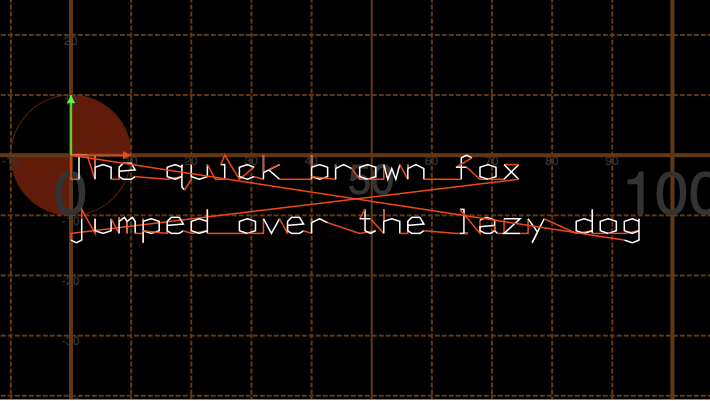
\includegraphics[width=0.35\textwidth]{src/Screenshot 2024-12-11 at 21.19.08.png}\\ \hline
        main & normal operation & test.txt, 10mm & 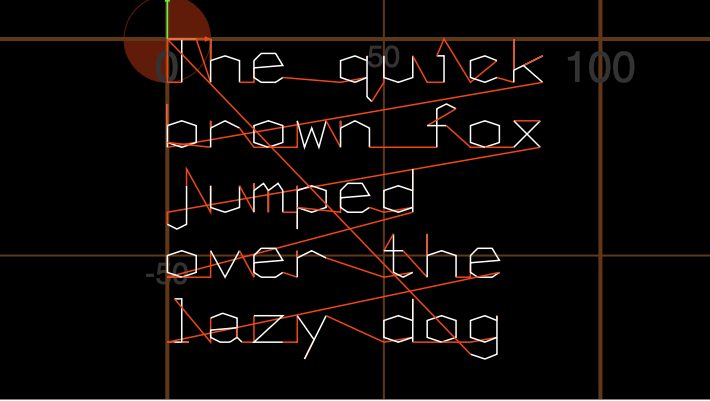
\includegraphics[width=0.35\textwidth]{src/Screenshot 2024-12-11 at 21.27.58.png}\\ \hline
        main & normal operation & test.txt, 6.56mm & 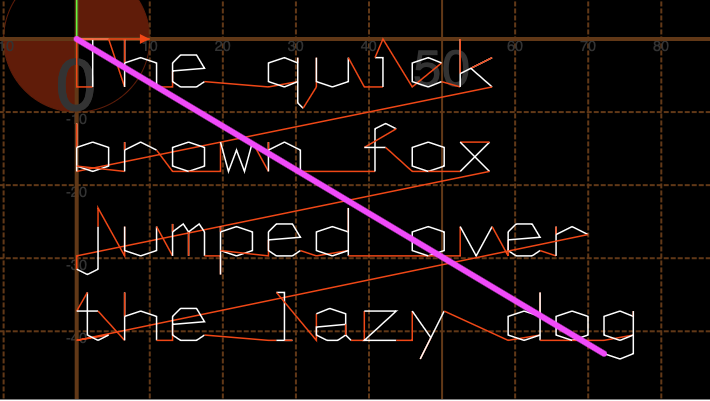
\includegraphics[width=0.35\textwidth]{src/Screenshot 2024-12-11 at 21.55.33.png}\\ \hline
        main & normal operation & RobotTesting.txt, 8mm & 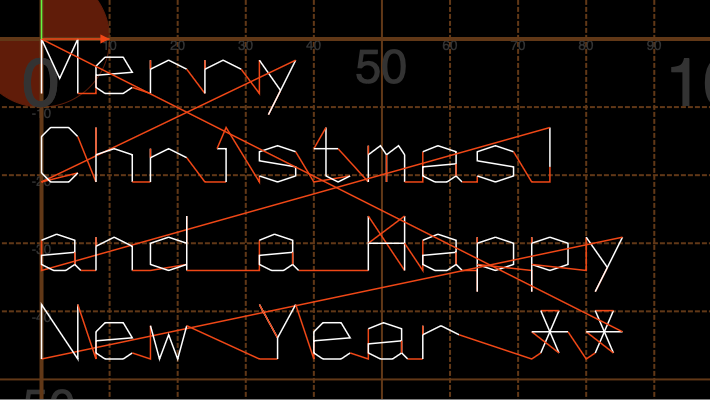
\includegraphics[width=0.35\textwidth]{src/Screenshot 2024-12-11 at 22.53.43.png}\\ \hline
        main & confirmation of correct scale & test.txt, 6.56mm & 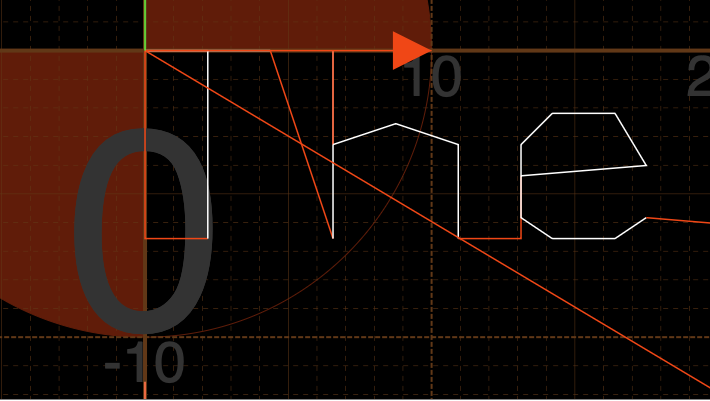
\includegraphics[width=0.35\textwidth]{src/Screenshot 2024-12-11 at 21.58.13.png}\\ \hline
        main & handling of large words and ** & test2.txt, "doggggggg", 10mm & 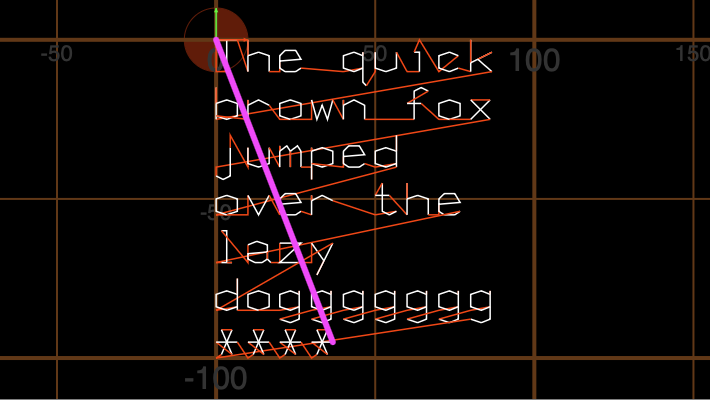
\includegraphics[width=0.35\textwidth]{src/Screenshot 2024-12-11 at 21.42.49.png}\\ \hline
        main & handling of very large words and ** & test2.txt, "dogggggggggg" , 10mm &  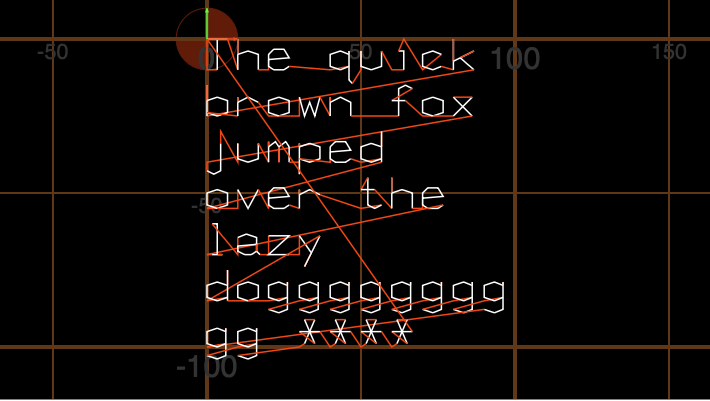
\includegraphics[width=0.35\textwidth]{src/Screenshot 2024-12-11 at 21.43.48.png} \\ \hline
        main & enforcment of $\backslash$n and $\backslash$r & test3.txt, 4mm &  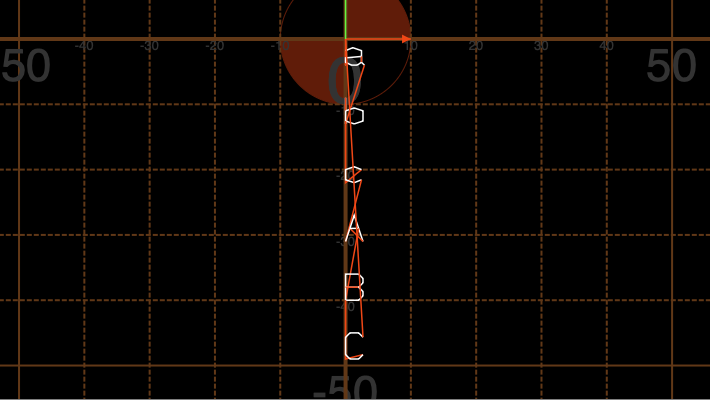
\includegraphics[width=0.35\textwidth]{src/Screenshot 2024-12-11 at 21.49.41.png} \\ \hline
        \end{longtable}

      